\chapter{Ordinary Differential Equations}


In Exercise~\ref{ex:duck}, we found the equilibrium point where a duck would float on water.  This kind of problem is called \emph{static} because it does not move.  This chapter introduces \emph{dynamic} problems, which involve things that change over time.

Also, you'll learn about a mathematical tool for describing physical systems, \emph{differential equations}, and two computational tools for solving them, Euler's method and \lstinline{ode45}.

But first I have a quick suggestion about organizing code in files.

\section{Functions and Files}
\label{funfiles}

So far we've only put one function in each file.  It's also possible
to put more than one function in a file, but only the first one, the
\emph{main function}, can be called from the Command
Window.  The other \emph{local functions} can be called from anywhere inside the file, but not from the Command Window or any other file.

\index{function!main}
\index{main function}
\index{local function}
\index{function!local}

Keeping multiple functions in one file is convenient, but it makes  debugging
difficult because you can't call local functions from the Command
Window.

To help with this problem, I often use the top-level function
to develop and test my local functions.  For example, to write
a program for Exercise~\ref{ex:duck}, I would create a file named
\emph{duck.m} and start with a main function named \lstinline{duck}
that takes no input variables and returns no output value.

Then I would write a function named \lstinline{error_func} to
evaluate the error function for \lstinline{fzero}.  To test
\lstinline{error_func}, I would call it from \lstinline{duck} and then
call \lstinline{duck} from the Command Window.

\index{incremental development}

Here's what my first draft might look like:

\begin{code}
function res = duck()
    error = error_func(10)
end

function res = error_func(d)
    rho = 0.3;      % density in g / cm^3
    r = 10;         % radius in cm
    res = d;
end
\end{code}

This program is not complete, but it is enough code to test.
Once this program is working, I would finish writing \lstinline{error_func}.
And once I'd finished and tested \lstinline{error_func}, I would modify
\lstinline{duck} to use \lstinline{fzero}.

This problem might only require two functions, but if there
were more, I could write and test them one at a time and then
combine them into a working program.

Now, let's get back to differential equations.


\section{Differential Equations}
\label{diffeq}

A \emph{differential equation (DE)} is an equation that describes the
derivatives of an unknown function.  ``Solving a DE'' means finding a
function whose derivatives satisfy the equation.

\index{differential equation}
\index{equation!differential}

For example, suppose we would like to predict the population of yeast growing in a nutrient solution.  Assume that we know the initial population is 5 billion yeast cells.
When yeast grow in particularly yeast-friendly
conditions, the rate of growth at any point in time is proportional to the current population.  If we define $y(t)$ to be the population at a time $t$, we can write the following equation for the rate of growth:
%
\begin{equation*}
\frac{dy}{dt}(t) = a y(t)
\end{equation*}
%
where $\frac{dy}{dt}(t)$ is the derivative of $y(t)$ and
$a$ is a constant that characterizes how quickly the population
grows.
This equation is \emph{differential} because it relates a function to one of its derivatives.

\index{ordinary differential equation (ODE)}
\index{partial differential equation (PDE)}

It is an \emph{ordinary differential equation (ODE)} because all the
derivatives involved are taken with respect to the
same variable.
If it related derivatives with respect to
different variables (partial derivatives), it would be a \emph{partial
differential equation (PDE)}.

\index{differential equation!first-order}

This equation is \emph{first order} because it involves only first
derivatives.  If it involved second derivatives, it would be second order,
and so on.

\index{linear differential equation}

Lastly, it's \emph{linear} because each term involves $t$, $y$, or
$dy/dt$ raised to the first power; if any of the terms involved
products or powers of $t$, $y$, or $dy/dt$ it would be
\emph{nonlinear}.

Now suppose we want to predict the yeast population in the future.  We can do that using Euler's method.

\section{Euler's Method}

Here's a test to see if you're as smart as Leonhard Euler.  Let's say you arrive at time (~$t$) and measure the current population ($y$) and
the rate of change ($r$).  What do you think the population will
be after some period of time $\Delta t$  has elapsed?

If you said $y + r \Delta t$, congratulations!  You just invented
Euler's method.

\index{Euler's method}

This estimate is based on the assumption that $r$ is constant, but in general it's not, so we only expect the estimate to be good if $r$ changes slowly and $\Delta t$ is small.

What if we want to make a prediction when $\Delta t$ is large?
One option is to break $\Delta t$ into smaller pieces, called
\emph{time steps}. Then we can use the following equations to get from one time step to the next:
\begin{equation}
    \label{e:euler}
    \begin{array}{r@{}l}
        tt_{i+1} &{}= tt_i + dt   \\
        yy_{i+1} &{}= yy_i + \frac{df}{dt}(t) \, dt        
    \end{array}
\end{equation}

Here, $tt_i$ is a vector of times when we estimate the value of $y$, and $yy_i$ is the vector of estimates.
For each index $i$, $yy_i$ is an estimate of $y(tt_i)$.

\index{time step}

If the rate doesn't change too fast and the time step isn't
too big, Euler's method is accurate enough for most purposes.

%One
%way to check is to run it once with time step $dt$ and then run it
%again with time step $dt/2$.  If the results are the same, they are
%probably accurate, as . . .; otherwise, we can cut the time step again.


\section{Implementing Euler's Method}

As an example we'll use Euler's method to solve Equation~\ref{e:euler},
\[ \frac{dy}{dt}(t) = a y(t) \]
with the initial condition $y(0) = \SI{5}{cells}$  and
the growth parameter $a = \SI{0.2}{cells/hr}$.

\index{main function}

As a first step, create a file named \emph{euler.m} with a main function and a local function:

\begin{code}
function res = euler()
    tt(1) = 0;
    yy(1) = 5;
    r = rate_func(tt(1), yy(1))
end

function res = rate_func(t, y)
   a = 0.2;
   dydt = a * y;
   res = dydt;
end
\end{code}

In \lstinline{euler} we initialize the initial conditions and then call \lstinline{rate_func}, so called because it computes the rate of growth in the population.

\index{initial condition}

After testing these functions, we can add code to \lstinline{euler} to compute these difference equations:
\begin{eqnarray*}
tt_{i+1} &=&tt_i + \Delta t             \\
yy_{i+1} &=& yy_i + r \Delta t
\end{eqnarray*}
%
where $r$ is the rate of growth computed by \lstinline{rate_func}.
Listing~\ref{lst:euler_method} has the code we need:

\lstinputlisting[style=mcode, caption={A function implementing Euler's method}, label={lst:euler_method}]{../code/chap_odes/euler.m}

Before the loop, we create two vectors, \lstinline{tt} and \lstinline{yy}, and set the first element of each with the initial conditions;  \lstinline{dt}, which is the size of the time steps, is \SI{0.1}{hours}.

Inside the loop, we compute the growth rate based on the current time, \lstinline{tt(i)}, and population, \lstinline{tt(i)}.  You might notice that the rate depends only on population, but we pass time as an input variable anyway, for reasons you'll see soon.

After computing the growth rate, we add an element both \lstinline{tt} and \lstinline{yy}, increasing their length by one.  Then, when the loop exits, we plot \lstinline{yy} as a function of \lstinline{tt}, adding labels and units as good engineering practice.

If you run the code, you should get a plot of population over time, as shown in Figure~\ref{fig:euler}.

\begin{figure}[ht!]
\centerline{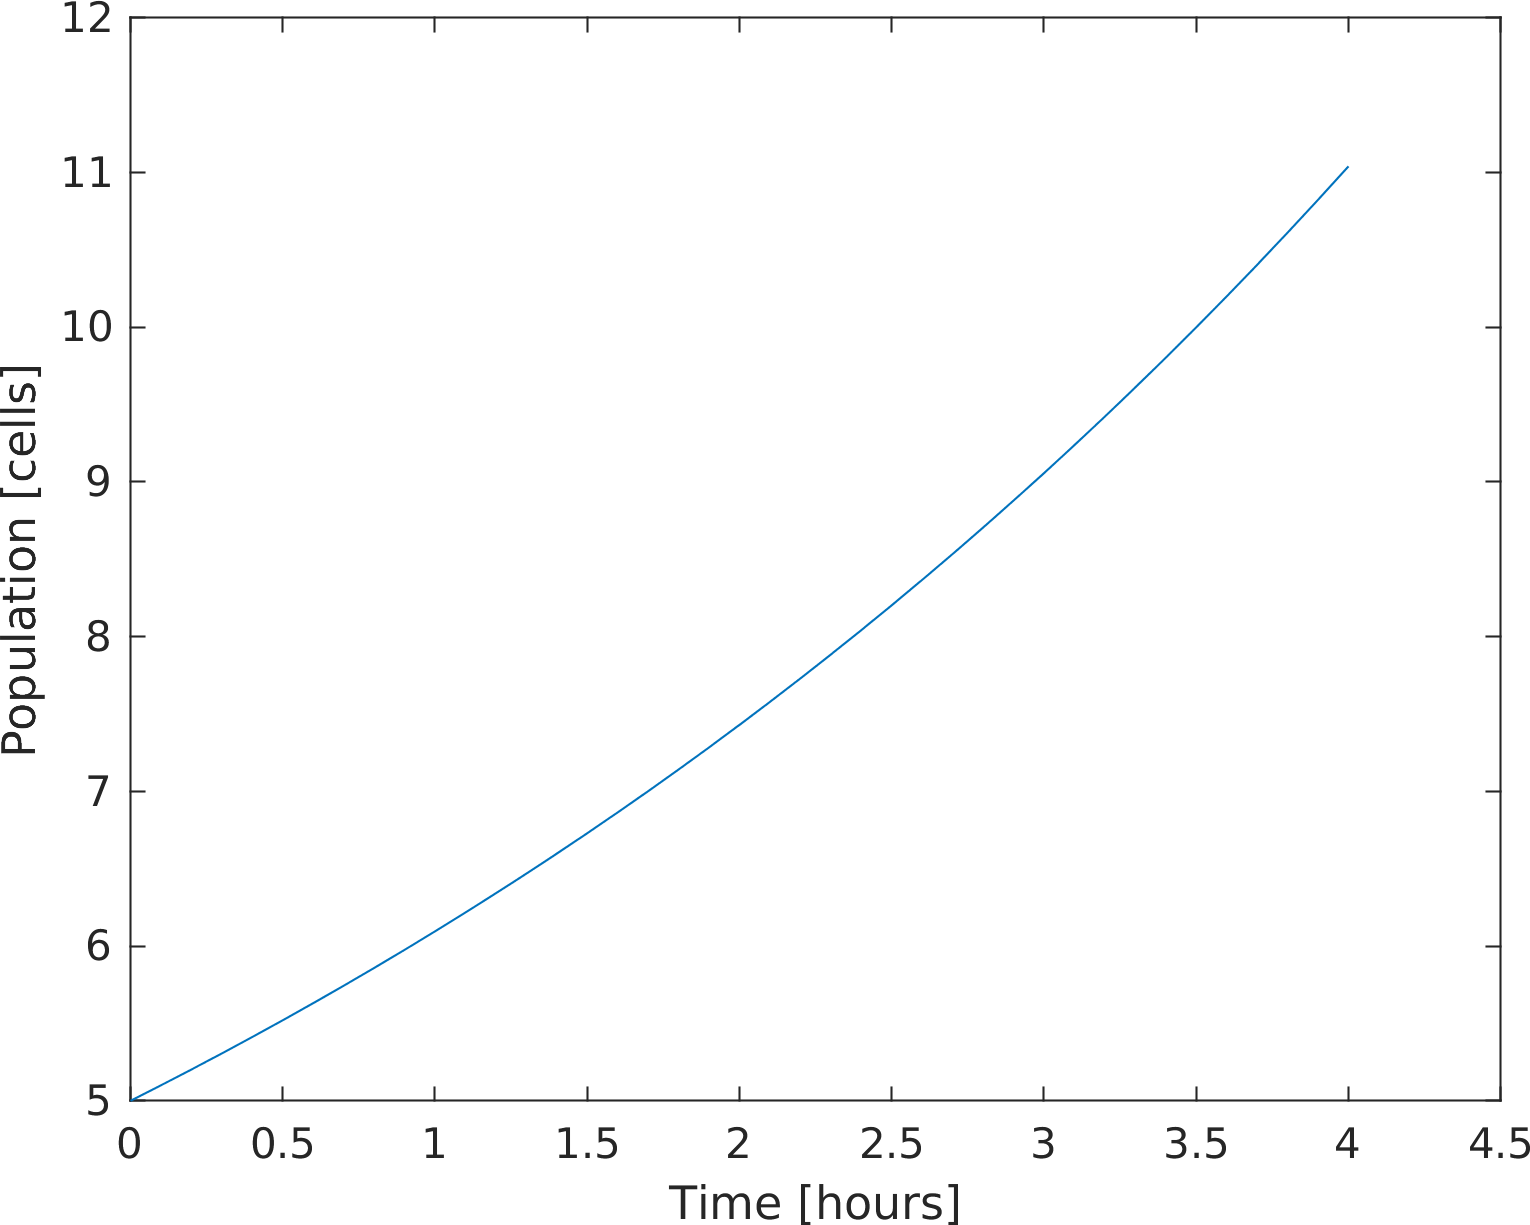
\includegraphics[width=0.7\textwidth]{images/euler.png}}
\caption{Solution to a simple differential equation by Euler's method}
\label{fig:euler}
\end{figure}

As you can see, the population doubles in a little less than 4 hours.  (You may recall for differential equations that for a linear, first-order system, the doubling time is $t_d = \ln(2)/r  = \ln(2)/0.2 = \SI{3.5}{s}$.)

\clearpage

\section{Solving ODEs with ode45}
\label{ode45}

A limitation of Euler's method is that it assumes that the derivative is constant between time steps, and that's not generally true.  Fortunately, there are better methods that estimate the derivative between time steps, and  they can be much more accurate.

\index{time step}
\index{ode45@\lstinline{ode45}}

MATLAB provides a function called \lstinline{ode45} that implements one of these methods.  In this section I'll explain how to use it; you can read more about how it works in Section~\ref{s:howode45} on page~\pageref{s:howode45}.

\index{rate function}
\index{function!rate}

In order to use \lstinline{ode45}, you have to write a function that evaluates $dy/dt$ as a function of $t$ and $y$.  Fortunately, we already have one, called \lstinline{rate_func}:

\begin{code}
function res = rate_func(t, y)
   a = 0.2;
   dydt = a * y;
   res = dydt;
end
\end{code}

We can call \lstinline{ode45} from the Command Window like this:

\begin{code}
[T, Y] = ode45(@rate_func, [0, 4], 5);
plot(T, Y)
\end{code}

The first argument is a function handle, as we saw in Chapter~\ref{fzero}.  The second argument is the time interval where we want to evaluate the solution; in this case the interval is from $t=0$ to $t=4$ hours.  The third argument is the initial population, 5 cells.  The result is two vectors, a vector of time values for the solution and a vector of the same length with the solution.

\index{function handle}
\index{handle!function}
\index{output variable}
\index{variable!output}

The full example, as a live script, is as follows:
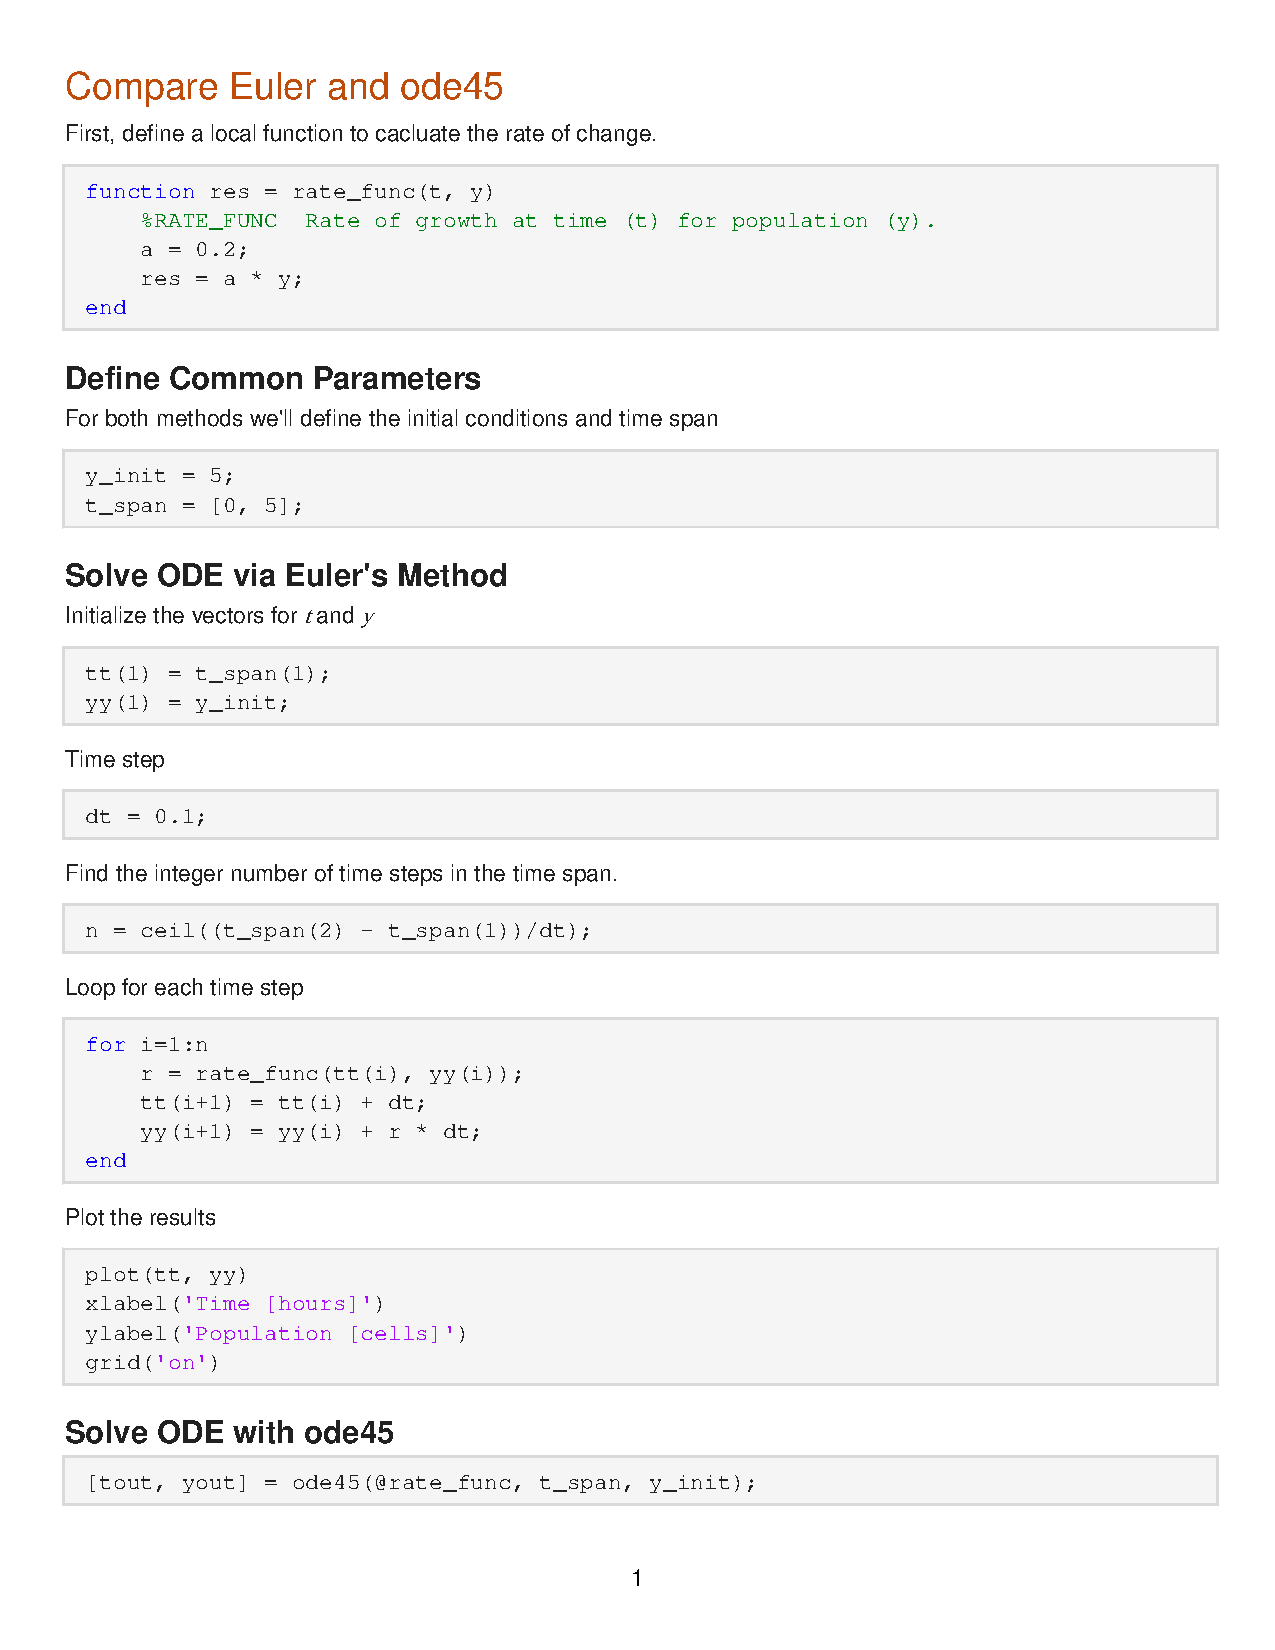
\includepdf[pages=-,frame,pagecommand={},width=\textwidth]{../code/chap_odes/euler_compare.pdf}

The solid line is the estimate we computed with Euler's method; the dashed line is the solution from \lstinline{ode45}.

For the first 2--3 hours, the two solutions are visually indistinguishable.  During the last hour, they diverge slightly; at 4 hours, the difference is less than 1 percent.

For many purposes, the difference between Euler's method and \lstinline{ode45} is the least of our worries.  In this example, we probably don't know the initial population with perfect accuracy or the growth constant, \lstinline{a}.  Also, the assumption that the growth rate only depends on population is probably not true.  Any of these modeling errors could be bigger than 1 percent.

However, for some problems, Euler's method can be off by a lot more than 1 percent.
In those cases \lstinline{ode45} is almost always more accurate, for two reasons: first, it computes the rate function several times per time step; second, if the time step is too big, \lstinline{ode45} can detect the problem and shrink the time step.  For more details, see ``\nameref{s:howode45}'' on page~\pageref{s:howode45}.


\section{Time Dependence}

Looking at \lstinline{rate_func} in the previous section, you might notice that it takes \lstinline{t} as an input variable but doesn't use it.  That's because the growth rate does not depend on time---bacteria don't know what time it is.

\index{time dependence}

But rats do.  Or, at least, they know what season it is.
Suppose that the growth rate for rats depends on the current population \emph{and} the availability of food, which varies over the course of the year.
The differential equation might be something like
%
\begin{equation*}
\frac{dy}{dt}(t) = a y(t) \left(1 - \cos (\omega t) \right)
\end{equation*}
%
where $t$ is time in days and $y(t)$ is the population at time $t$.
Because the growth rate depends on time, this differential equation is \emph{time dependent}.

The variables $a$ and $\omega$ are \emph{parameters}, which are values that
quantify a physical aspect of the scenario.  Parameters are often constants, but in some models they vary in time.

\index{parameter}

In this example, $a$ characterizes the reproductive rate per day, and
$\omega$ is the frequency of a periodic function that describes
the effect of varying food supply on reproduction.

We'll use the values $a = \SI{0.002}{day^{-1}}$
and $\omega = 2 \pi / 365 \SI{}{rad/day}$ (one cycle per year).
The growth rate is lowest at $t=0$, on January~1, and highest at $t=365/2$, on June~30.

Now we can write a function that evaluates the growth rate:

\begin{code}
function res = rate_func(t, rats)
    %RATE_FUNC returns the growth rate at time (t) for population (rats)
    a = 0.002;
    omega = 2*pi / 365;
    res = a * rats * (1 - cos(omega * t));
end
\end{code}

To test this function, I put it in a file called \emph{rats.m} with a main function called
\lstinline{rats}:

\begin{code}
function res = rats_growth()
    t = 365/2;
    rats = 1000;
    res = rate_func(t, rats);
end
\end{code}

The main function assumes, for purposes of testing, that
there are 1000 rats at $t=365/2$ (June~30) and computes the growth rate under those conditions.

We can run the main function like this:

\begin{code}
>> r = rat_growth()

r = 4
\end{code}

Under these conditions, the growth rate is 4 new rats per day.

Now that we've tested \lstinline{rate_func}, we can use \lstinline{ode45} to solve the differential equation.
Here's how to call it from the main function in \emph{rats.m}:

\begin{code}
[tt, yy]] = ode45(@rate_func, [0, 365], 1000)
plot(tt, yy)
\end{code}

The first argument is a function handle, again.  The second argument is the interval we are interested in, a duration of one year, expressed in units of days.
The third argument is the initial population, $y(0) = 1000$.

\index{interval}

We can put this all together in the following program:
\lstinputlisting[style=mcode]{../code/chap_odes/rat_growth.m}

Figure~\ref{fig:rats} shows the results.

\begin{figure}[ht]
\centerline{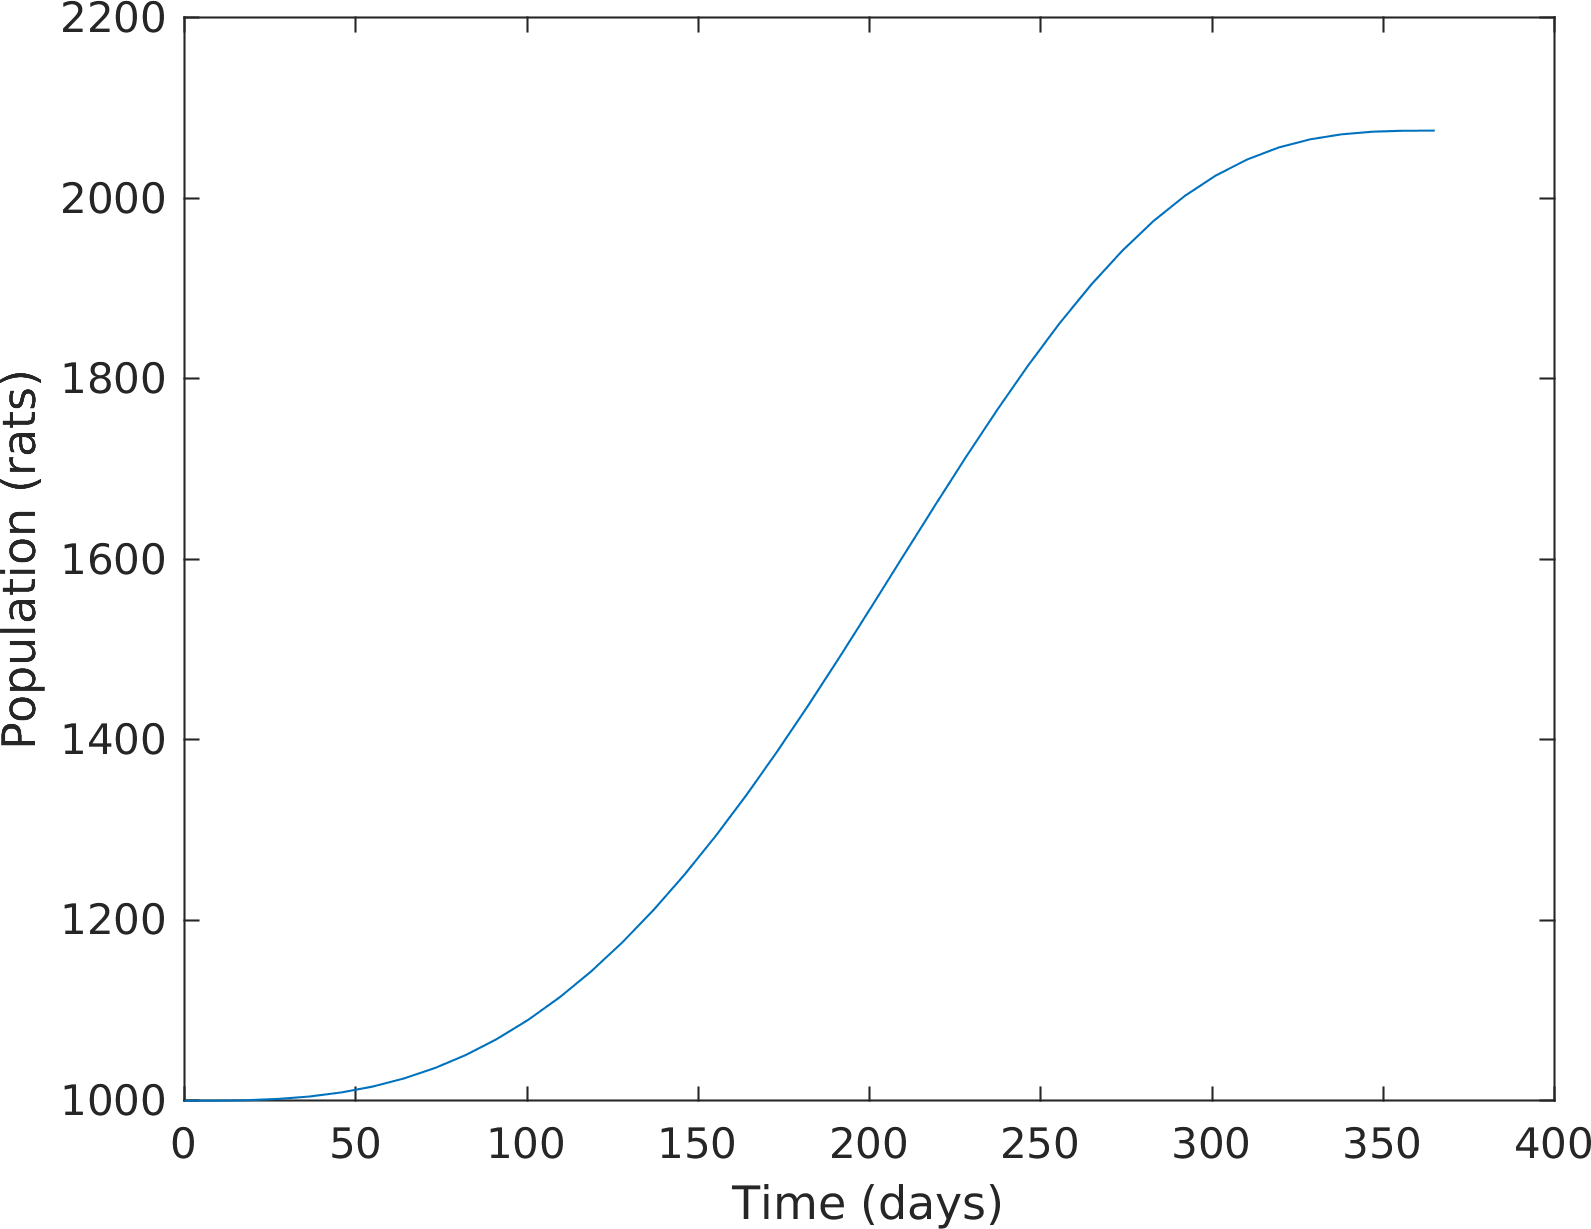
\includegraphics[width=0.7\textwidth]{../code/chap_odes/rats.png}}
\caption{Solutions to a time-dependent differential equation by Euler's method and \lstinline{ode45}}
\label{fig:rats}
\end{figure}

The population grows slowly during the winter, quickly during the summer, and then slowly again in the fall.

To see the population at the end of the year, you can display the last element of \lstinline{rats}:

\begin{code}
rats(end)
2.0751e+03
\end{code}

That's a little more than 2000 rats, so the population roughly doubles in one year.

The index here is \lstinline{end}, which is a special word in MATLAB that means ``the index of the last element.''  You can use it in an expression, so \lstinline{Y(end - 1)} is the second-to-last element of
\lstinline{Y}.

\index{end statement@\lstinline{end} statement}
\index{index!end@\lstinline{end}}


\section{What Could Go Wrong?}

Don't forget the \lstinline{@} on the function handle.
If you leave it out, like:

\begin{code}
[tt, yy] = ode45(rate_func, [0, 365], 1000)
\end{code}
MATLAB treats the first argument as a function
call and calls \lstinline{rate_func} without providing arguments.
Then you get an error message:

\index{rate function}
\index{function handle}

\begin{code}
Not enough input arguments.

Error in rats>rate_func (line 18)
    res = a * y * (1 - cos(omega * t));

Error in rats (line 6)
    [tt, yy] = ode45(rate_func, [0, 365], 1000);
\end{code}

Also, the rate function you write has to take two input variables,
\lstinline{t} and \lstinline{y}, in that order, and return one output variable,
\lstinline{res}.

\index{output variable}

If you're working with a rate function like:

\begin{equation*}
\frac{dy}{dt}(t) = a y(t)
\end{equation*}
you might be tempted to write this:

\begin{code}
function res = rate_func(y)        % WRONG
    a = 0.002;
    res = a * y;
end
\end{code}

But that would be wrong.  So very wrong.  Why?  Because
when \lstinline{ode45} calls \lstinline{rate_func}, it provides two arguments.
If you only take one input variable, you'll get an error.  So
you have to write a function that takes \lstinline{t} as an input
variable, even if you don't use it:

\index{input variable}

\begin{code}
function res = rate_func(t, y)     % RIGHT
    a = 0.002;
    res = a * y;
end
\end{code}

Another common error is to write a function that doesn't make
an assignment to the output variable.  If you write something
like:

\begin{code}
function res = rate_func(t, y)
    a = 0.002;
    omega = 2*pi / 365;
    r = a * y * (1 - cos(omega * t));    % WRONG
end
\end{code}
 and then call it from \lstinline{ode45}, you get

\begin{code}
Output argument "res" (and maybe others) not assigned during call
to "rate_func".
\end{code}

I hope these warnings save you some time debugging.

\section{Labeling Axes}

The plots in this chapter have labels on the axes, and one of them has a legend, but I didn't show you how to do that.  Let's do it now.

\index{labeling axes}
\index{axes}
\index{xlabel@\lstinline{xlabel}}
\index{ylabel@\lstinline{ylabel}}

The functions to label the axes are \lstinline{xlabel} and \lstinline{ylabel}:

\begin{code}
xlabel('Time (hours)')
ylabel('Population (billions of cells)')
\end{code}

The function to generate a legend is \lstinline{legend}:

\begin{code}
legend('euler', 'ode45')
\end{code}

\index{legend@\lstinline{legend}}

The arguments are the labels for the lines, in the order they were drawn.  Usually the legend is in the upper-right corner, but you can move it by providing an optional argument called \lstinline{Location}:

\begin{code}
legend('euler', 'ode45', 'Location', 'northwest')
\end{code}

Finally,  save the figures using \lstinline{saveas}:

\begin{code}
saveas(gcf,'runge.png','png')
\end{code}

The first argument is the figure we want to save; \lstinline{gcf} is a MATLAB command that stands for ``get current figure,'' which is the figure we just drew.  The second argument is the filename.  The extension specifies the format we want, which is a PNG (\emph{.png}) image file.  The third argument tells MATLAB what driver to use.  The details aren't important, but \lstinline{'png'} generates figures as color images.

\index{figure}
\index{get current figure}
\index{gcf@\lstinline{gcf}}
\index{saveas@\lstinline{saveas}}


\section{How ode45 Works}
\label{s:howode45}

According to the MATLAB documentation, \lstinline{ode45} uses ``an explicit Runge-Kutta formula, the Dormand-Prince pair.''  You can read about it at  \url{https://greenteapress.com/matlab/runge}, but I'll give you a sense of it here.

\index{Runge-Kutta}
\index{ode45@\lstinline{ode45}}
\index{Dormand-Prince}

The key idea behind all Runge-Kutta methods is to evaluate the rate function several times at each time step and use a weighted average of the computed slopes to estimate the value at the next time step.
Different methods evaluate the rate function in different places and compute the average with different weights.

\index{differential equation}
\index{rate function}
\index{function!rate}

As an example, we'll solve the following differential equation:

\[ \frac{dy}{dt}(t) = y \sin t \]

Given a differential equation, it's usually straightforward to write a rate function:

\begin{code}
function res = rate_func(t, y)
    dydt = y * sin(t);
    res = dydt;
end
\end{code}

And we can use it like this:

\begin{code}
    y0 = 1;
    tspan=[0 4];
    options = odeset('Refine', 1);
    [T, Y] = ode45(@rate_func, tspan, y0, options);
\end{code}

For this example we'll use \lstinline{odeset} to set the \lstinline{Refine} option to \lstinline{1}, which tells \lstinline{ode45} to return only the time steps it computes, rather than interpolating between them.

\index{odeset@\lstinline{odeset}}

Now we can modify the rate function to plot the places where it gets evaluated:

\begin{code}
function res = rate_func(t, y)
    dydt = y * sin(t);
    res = dydt;

    plot(t, y, 'ro')
    dt = 0.01;
    ts = [t t+dt];
    ys = [y y+dydt*dt];
    plot(ts, ys, 'r-')
end
\end{code}

When \lstinline{rate_func} runs, it plots a red circle at each location and a short red line showing the computed slope.

\index{time step}

Figure~\ref{fig:odeplot1} shows the result;  \lstinline{ode45} computes 10 time steps (not counting the initial condition) and evaluates the rate function 61 times.

\begin{figure}[h]
\centerline{\includegraphics[scale=0.8]{images/figure15_01_new.eps}}
\caption{Points where \lstinline{ode45} evaluates the rate function}
\label{fig:odeplot1}
\end{figure}

Figure~\ref{fig:odeplot2} shows the same plot, zoomed in on a single time step.
The dark squares at $0.8$ to $1.2$ show the values that were returned as part of the solution.
The circles show the places where the rate function was evaluated.

\begin{figure}[h]
\centerline{\includegraphics[scale=0.8]{images/figure15_02_new.eps}}
\caption{Points where \lstinline{ode45} evaluates the rate function, zoomed in}
\label{fig:odeplot2}
\end{figure}

We can see that \lstinline{ode45} evaluates the rate function several times per time step, at several places between the end points.
We can also see that most of the places where \lstinline{ode45} evaluates the rate function are not part of the solution it returns, and they are not always good estimates of the solution.
This is good to know when you are writing a rate function; you should not assume that the time and state you get as input variables will be part of the solution.

In a sense, the rate function is answering a hypothetical question: ``\emph{If} the state at a particular time has these particular values, what \emph{would} the slope~be?''


At each time step, \lstinline{ode45} actually computes \emph{two} estimates of the next value.
By comparing them, it can estimate the magnitude of the error,  which it uses to adjust the time step.
If the error is too big, it uses a smaller time step; if the error is small enough, it uses a bigger time step.
Because \lstinline{ode45} is \emph{adaptive} in this way, it minimizes the number of times it calls the rate function to achieve a given level of accuracy.

\index{adaptive}



\section{Chapter Review}

This chapter introduced \emph{differential equations (DE)}, which are equations that describe the
derivatives of an unknown function.
In an \emph{ordinary differential equation (ODE)}, all derivatives are taken with
respect to the same variable, as opposed to a \emph{partial differential equation (PDE)}, which includes derivatives with respect to more than one variable.

A \emph{first-order DE} includes only first derivatives, and a \emph{linear DE} includes no products or powers of the function and its derivatives.
A differential equation is \emph{time dependent} if the rate function depends on time.

When we solve a differential equation numerically, the \emph{time step} is the interval in time between successive elements of the solution.
A \emph{parameter} is a value that appears in a model to quantify some
physical aspect of the scenario being modeled.

Until now, we have only put one function in each M-file, but in this chapter we wrote a \emph{main function}, which is the first function in an M-file, and a \emph{local function}, which is any function in an M-file that is not the main function.

In the next chapter, we'll solve \emph{systems} of ODEs, which are used to describe physical systems with multiple parts that interact.
But first, here's an exercise where you can apply what you've learned so far.


\section{Exercise}

Before you go on, you might want to work on the following exercise.

\begin{ex}

\index{coffee}
\index{cooling}
\index{Newton's law of cooling}

Suppose that you're given an 8-ounce cup of coffee at \SI{90}{\celsius}.
You have learned from bitter experience that the hottest coffee you
can drink comfortably is \SI{60}{\celsius}.

If the temperature of the coffee drops by \SI{0.7}{\celsius} during the first minute, how long will you have to wait to drink your coffee?

You can answer this question with Newton's Law of Cooling (see  \url{https://greenteapress.com/matlab/newton}):
%
\begin{equation*}
\frac{dy}{dt}(t) = -k (y(t) - e)
\end{equation*}
%
where $y(t)$ is the temperature of the coffee at time $t$,
$e$ is the temperature of the environment, and $k$ is a parameter
that characterizes the rate of heat transfer from the coffee to the environment.

Let's assume that $e$ is \SI{20}{\celsius} and constant; that is, the coffee does not warm up the room.

Let's also assume $k$ is constant.  In that case, we can estimate it based on the information we have.  If the temperature drops \SI{0.7}{\celsius} during the first minute, when the coffee is \SI{90}{\celsius}, we can write
%
\begin{equation*}
-0.7 = -k (90 - 20)
\end{equation*}
%

Solving this equation yields $k = 0.01$.

Here are some suggestions for getting started:

\begin{enumerate}

\item Create a file named \emph{coffee.m} and write a function
called \lstinline{coffee} that takes no input variables.  Put a simple statement like \lstinline{x = 5} in the body of the function and invoke \lstinline{coffee} from the Command  Window.

\item Add a helper function called \lstinline{rate_func} that takes \lstinline{t} and \lstinline{y} and computes $dy/dt$.  In this case, \lstinline{rate_func} does not actually depend on $t$; nevertheless, your function has to take $t$ as the first input variable in order to work with \lstinline{ode45}.

\item Test your function by adding a line like \lstinline{rate_func(0, 90)}
to \lstinline{coffee}, then call \lstinline{coffee} from the Command Window.
Confirm that the initial rate is \SI{-0.7}{\celsius \per \minute}.

\item Once you get \lstinline{rate_func} working, modify
\lstinline{coffee} to use \lstinline{ode45} to compute the temperature
of the coffee for 60 minutes.  Confirm that
the coffee cools quickly at first, then cools more slowly, and reaches
room temperature after about an hour.

\item Plot the results and estimate the time when the temperature reaches~\SI{60}{\celsius}.

\end{enumerate}

\end{ex}
